% A Baker's Dozen -- twelve solved examples from Symbulator 9's
% documentation, and a bonus. GENERATED by build_dozen_tex.py from the data
% in build_dozen.py; edit that, not this. Compile with XeLaTeX.
\documentclass[10pt]{article}
\usepackage[a4paper,top=16mm,bottom=16mm,left=17mm,right=17mm]{geometry}
\usepackage{fontspec}
\setmainfont{IBM Plex Serif}
\setsansfont{IBM Plex Sans}
\setmonofont{IBM Plex Mono}[Scale=0.88]
\newfontfamily\anglefont{DejaVuSansMono.ttf}[Scale=0.88]
\usepackage{amsmath,amssymb}
\usepackage{newunicodechar}
\newunicodechar{Ω}{\ensuremath{\Omega}}
\newunicodechar{ω}{\ensuremath{\omega}}
\newunicodechar{Δ}{\ensuremath{\Delta}}
\newunicodechar{∠}{{\anglefont ∠}}
\usepackage[table]{xcolor}
\definecolor{navy}{HTML}{203864}
\definecolor{accent}{HTML}{2F5FA8}
\definecolor{accentbg}{HTML}{E9EFF8}
\definecolor{ink2}{HTML}{545D6D}
\definecolor{ink3}{HTML}{858D9C}
\definecolor{rule}{HTML}{E2E5EA}
\definecolor{answer}{HTML}{A13030}
\definecolor{gold}{HTML}{D9A521}
\definecolor{lcd}{HTML}{F2F6FC}
\definecolor{lcdedge}{HTML}{DBE4F2}
\usepackage{graphicx}
\usepackage[export]{adjustbox}
\usepackage{fancyvrb}
\usepackage[most]{tcolorbox}
\usepackage[siunitx]{circuitikz}
\usepackage{array}
\usepackage[hidelinks]{hyperref}
\urlstyle{tt}
\frenchspacing
\setlength{\parindent}{0pt}
\setlength{\parskip}{0pt}
\pagestyle{empty}

\newtcolorbox{whybox}{enhanced, breakable, colback=accentbg, boxrule=0pt,
  leftrule=1.1mm, colframe=accent, arc=0pt, outer arc=0pt,
  left=3mm, right=3mm, top=2mm, bottom=2mm, before skip=1mm, after skip=3mm}
\newtcolorbox{codebox}{colback=lcd, colframe=lcdedge, boxrule=0.4pt, arc=1.2mm,
  left=2.5mm, right=2.5mm, top=1.5mm, bottom=1.5mm, before skip=0.8mm, after skip=1.4mm}
\newtcolorbox{answerbox}{colback=white, colframe=answer, boxrule=0pt,
  leftrule=0.6mm, arc=0pt, outer arc=0pt, left=2.5mm, right=0mm, top=0.4mm,
  bottom=0.4mm, before skip=0.9mm, after skip=0.9mm, fontupper=\color{answer}}

\newcommand{\kicker}[1]{{\setlength{\fboxsep}{1.2mm}\colorbox{navy}{%
  \textcolor{white}{\sffamily\scriptsize\addfontfeature{LetterSpace=18}\MakeUppercase{#1}}}}}
% Not uppercased: a label like "TR, t > 0" carries a variable.
\newcommand{\runhead}[1]{{\sffamily\footnotesize\bfseries\color{accent}#1}\par\vspace{0.6mm}}
\newcommand{\settings}[1]{{\sffamily\footnotesize\color{ink2}#1}\par}
\newcommand{\applink}[1]{\vspace{0.6mm}{\scriptsize\color{accent}\url{#1}}\par}

\newenvironment{problem}[4]{%
  \newpage
  \kicker{#1}\par\vspace{2.5mm}
  {\sffamily\fontsize{20}{24}\selectfont\bfseries\color{navy}#2\par}
  \vspace{0.8mm}{\sffamily\large\color{accent}#3\par}
  \vspace{0.8mm}{\sffamily\footnotesize\color{ink3}#4\par}
  \vspace{1.5mm}{\color{gold}\rule{\linewidth}{0.7pt}}\par\vspace{3mm}
}{}

\begin{document}


{\setlength{\fboxsep}{3mm}\colorbox{navy}{
\includegraphics[width=20mm]{../../web/assets/logo.png}}}\par
\vspace{5mm}{\sffamily\small\bfseries\color{accent}\addfontfeature{LetterSpace=28}SYMBULATOR 9}\par
\vspace{3mm}{\sffamily\fontsize{40}{44}\selectfont\bfseries\color{navy}A Baker's Dozen\par}
\vspace{5mm}{\color{gold}\rule{38mm}{2.2mm}}\par
\vspace{4mm}{\sffamily\Large\color{ink2}Twelve solved examples from the documentation, and a bonus\par}
\vspace{7mm}\begin{minipage}{150mm}\large
Each of these circuits looks like an afternoon's work by hand. Symbulator solves each one in a single run, or in two when a switch splits the problem into intervals. No two of them make the same point. Every description below is the one in the app's built-in examples, and every answer was checked against the app on 16 September 2026. The link under each run opens the entry in the online app.
\end{minipage}\par
\vspace{8mm}{\sffamily\arrayrulecolor{rule}\renewcommand{\arraystretch}{1.55}%
\begin{tabular}{@{}p{9mm}p{72mm}p{85mm}@{}}\hline
\textcolor{accent}{\bfseries 1} & \textbf{AS7's Example 3.4} & \textcolor{ink2}{\small Supernodes around a dependent source} \\ \hline
\textcolor{accent}{\bfseries 2} & \textbf{NR12's Example 5.7} & \textcolor{ink2}{\small A realistic op amp model} \\ \hline
\textcolor{accent}{\bfseries 3} & \textbf{Bo2's Example 3.3} & \textcolor{ink2}{\small Two op amps, every conductance a symbol} \\ \hline
\textcolor{accent}{\bfseries 4} & \textbf{AS7's Problem 9.73} & \textcolor{ink2}{\small Eight impedances that will not reduce} \\ \hline
\textcolor{accent}{\bfseries 5} & \textbf{AS7's Example 10.14} & \textcolor{ink2}{\small Phasors with a dependent source} \\ \hline
\textcolor{accent}{\bfseries 6} & \textbf{AS7's Example 12.11} & \textcolor{ink2}{\small Three-phase wye-delta with line impedances} \\ \hline
\textcolor{accent}{\bfseries 7} & \textbf{AS7's Practice Problem 13.13} & \textcolor{ink2}{\small Coupled coils in a tangle} \\ \hline
\textcolor{accent}{\bfseries 8} & \textbf{NR11's switched RLC with coupled coils} & \textcolor{ink2}{\small A transient across a coupling} \\ \hline
\textcolor{accent}{\bfseries 9} & \textbf{Bo2's Drill Exercise 6.6} & \textcolor{ink2}{\small Two capacitors around an op amp} \\ \hline
\textcolor{accent}{\bfseries 10} & \textbf{Prof. Boulet's exam problem} & \textcolor{ink2}{\small The switch, the ladder and the damped sine} \\ \hline
\textcolor{accent}{\bfseries 11} & \textbf{AS7's Problem 19.2} & \textcolor{ink2}{\small A two-port with no ground} \\ \hline
\textcolor{accent}{\bfseries 12} & \textbf{NR12's Example 18.6} & \textcolor{ink2}{\small Two amplifiers known only by their h parameters} \\ \hline
\textcolor{gold}{\bfseries$\bigstar$} & \textbf{A freebie, on the house} & \textcolor{ink2}{\small One dependent source of each kind} \\ \hline
\end{tabular}}

\begin{problem}{Sample 1 of 12}{AS7's Example 3.4}{Supernodes around a dependent source}{Alexander \& Sadiku sampler}
{\itshape Find the node voltages in the circuit of the figure.\par}
\vspace{1mm}
\begin{center}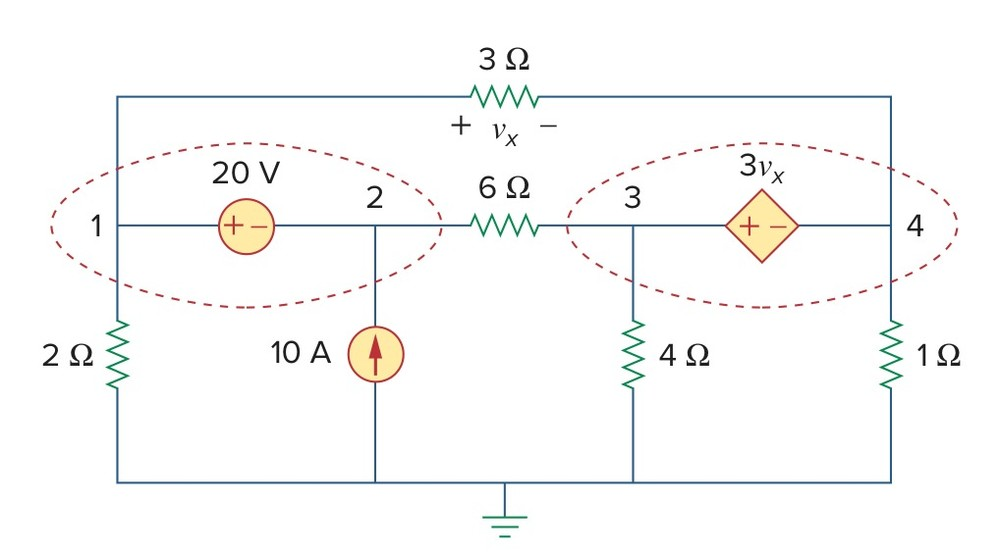
\includegraphics[width=111.5mm,max width=\linewidth]{../../assets/circuit/as7-ex3-4.jpg}\end{center}
\begin{whybox}\textbf{\sffamily\color{navy}Why it is here.} Two voltage sources float between non-reference nodes, and one of them is worth three times the drop across a resistor. By hand that is two supernodes and a constraint equation. Here it is eight lines typed as they are drawn.\end{whybox}
\runhead{DC}
\begin{codebox}
\begin{Verbatim}[fontsize=\small]
e1,1,2,20
r3,1,4,3
r6,2,3,6
e2,3,4,3*vr3
r2,1,0,2
j,0,2,10
r4,3,0,4
r1,4,0,1
\end{Verbatim}
\end{codebox}
\settings{Analysis: DC. Rounding: approx.}
\begin{answerbox}
\adjustbox{max width=\linewidth}{$\displaystyle v_{1} = 26.667\ \mathrm{V}$}
\end{answerbox}
\begin{answerbox}
\adjustbox{max width=\linewidth}{$\displaystyle v_{2} = 6.6667\ \mathrm{V}$}
\end{answerbox}
\begin{answerbox}
\adjustbox{max width=\linewidth}{$\displaystyle v_{3} = 173.33\ \mathrm{V}$}
\end{answerbox}
\begin{answerbox}
\adjustbox{max width=\linewidth}{$\displaystyle v_{4} = -46.667\ \mathrm{V}$}
\end{answerbox}
\applink{https://symbulator.pythonanywhere.com/?lesson=as7&entry=2}
\end{problem}

\begin{problem}{Sample 2 of 12}{NR12's Example 5.7}{A realistic op amp model}{Nilsson \& Riedel sampler}
{\itshape Analyze the noninverting amplifier using the realistic op amp model, with open-loop gain $A$ = 50,000, input resistance $R_i$ = 100 kΩ and output resistance $R_o$ = 7.5 kΩ. Find the gain $v_o/v_g$.\par}
\vspace{1mm}
\begin{center}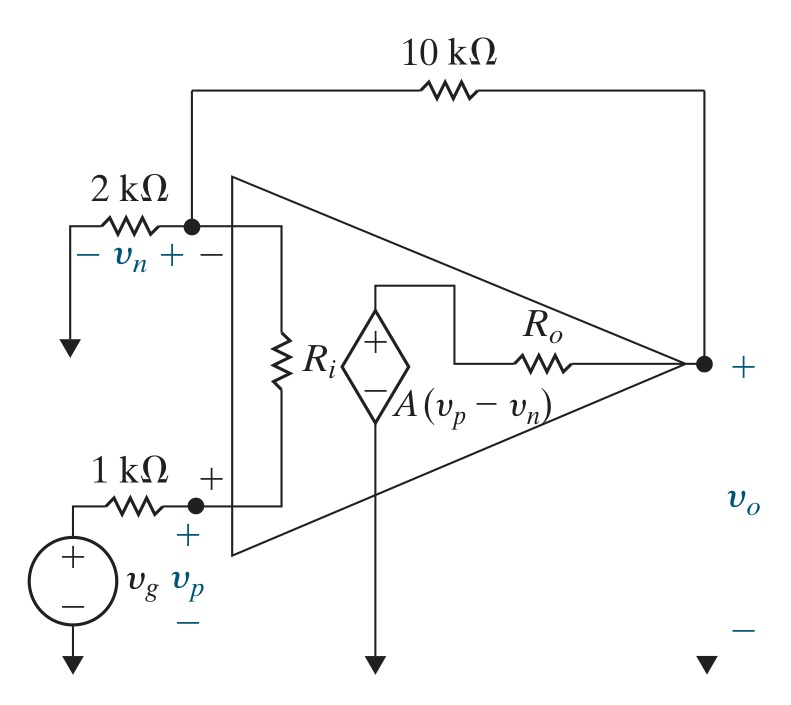
\includegraphics[width=69.6mm,max width=\linewidth]{../../assets/circuit/nr12-ex5-7.jpg}\end{center}
\begin{whybox}\textbf{\sffamily\color{navy}Why it is here.} The model is a dependent source with a finite gain, an input resistance and an output resistance, written as three ordinary elements. The source stays a symbol, so the gain is read straight off the answer.\end{whybox}
\runhead{DC}
\begin{codebox}
\begin{Verbatim}[fontsize=\small]
eg,1,0,vg
rg,1,p,1'k
ri,p,n,100'k
rs,n,0,2'k
rf,n,3,10'k
ro,4,3,7.5'k
ea,4,0,50000*(vp-vn)
\end{Verbatim}
\end{codebox}
\settings{Analysis: DC. Rounding: approx. Evaluate: v\_3/vg.}
\begin{answerbox}
\adjustbox{max width=\linewidth}{$\displaystyle v_{3}/v_{g} = 5.9988$}
\end{answerbox}
\applink{https://symbulator.pythonanywhere.com/?lesson=nr12&entry=14}
\end{problem}

\begin{problem}{Sample 3 of 12}{Bo2's Example 3.3}{Two op amps, every conductance a symbol}{Course, Lesson 5 (Operational Amplifiers)}
{\itshape Find $v_o$ in terms of the conductances and the applied voltage $v_S$.\par}
\vspace{1mm}
\begin{center}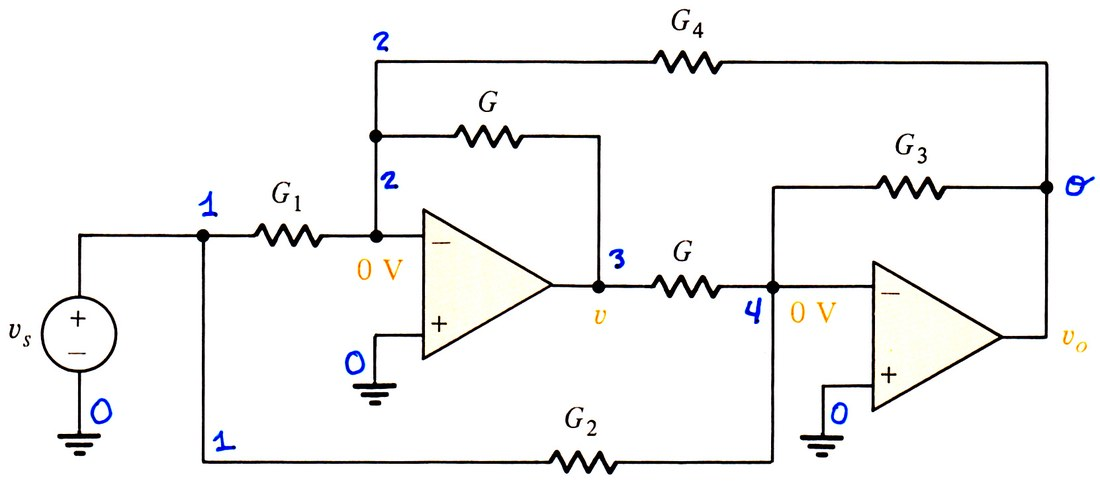
\includegraphics[width=141.8mm,max width=\linewidth]{../../assets/practice/bo2s-example-3-3-cascade-37.jpg}\end{center}
\begin{whybox}\textbf{\sffamily\color{navy}Why it is here.} There is not a single number in the circuit. The answer is the gain as a formula, and its shape explains the circuit: a difference of conductances over a difference of conductances.\end{whybox}
\runhead{DC}
\begin{codebox}
\begin{Verbatim}[fontsize=\small]
e,1,0,vs
r12,1,2,1/g1
r14,1,4,1/g2
r4o,4,o,1/g3
r2o,2,o,1/g4
r23,2,3,1/g
r34,3,4,1/g
o1,0,2,3
o2,0,4,o
\end{Verbatim}
\end{codebox}
\settings{Analysis: DC. Rounding: exact.}
\begin{answerbox}
\adjustbox{max width=\linewidth}{$\displaystyle v_{o} = \dfrac{(g_{1} - g_{2})\,v_{s}}{g_{3} - g_{4}}$}
\end{answerbox}
\applink{https://symbulator.pythonanywhere.com/?lesson=5b&entry=14}
\end{problem}

\begin{problem}{Sample 4 of 12}{AS7's Problem 9.73}{Eight impedances that will not reduce}{Course, Lesson 7 (AC)}
{\itshape Determine the equivalent impedance for the circuit.\par}
\vspace{1mm}
\begin{center}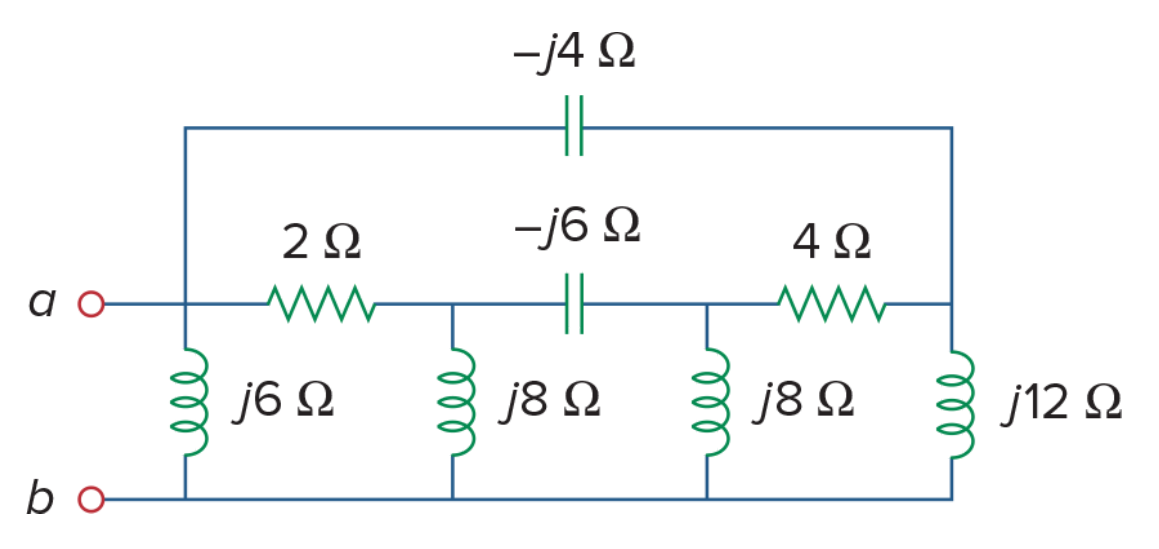
\includegraphics[width=130.9mm,max width=\linewidth]{../../assets/circuit/as7p0973.png}\end{center}
\begin{whybox}\textbf{\sffamily\color{navy}Why it is here.} No two of these impedances are in series or in parallel, so by hand the circuit needs a delta-wye transformation. Find equivalent does it in one run.\end{whybox}
\runhead{AC}
\begin{codebox}
\begin{Verbatim}[fontsize=\small]
r10,1,0,6j
r20,2,0,8j
r30,3,0,8j
r40,4,0,12j
r12,1,2,2
r23,2,3,-6j
r34,3,4,4
r14,1,4,-4j
\end{Verbatim}
\end{codebox}
\settings{Analysis: Find equivalent, Resistance / impedance, between nodes 1 and 0, in AC. ω = 1 (any value gives the same answer, every impedance being in ohms). Rounding: 4 digits.}
\begin{answerbox}
\adjustbox{max width=\linewidth}{$\displaystyle Z_{eq} = 0.3794 + 1.46\,\mathrm{j}\ \Omega$}
\end{answerbox}
\applink{https://symbulator.pythonanywhere.com/?lesson=7&entry=6}
\end{problem}

\begin{problem}{Sample 5 of 12}{AS7's Example 10.14}{Phasors with a dependent source}{Course, Lesson 7 (AC)}
{\itshape Find $V_1$ and $V_2$ in the circuit.\par}
\vspace{1mm}
\begin{center}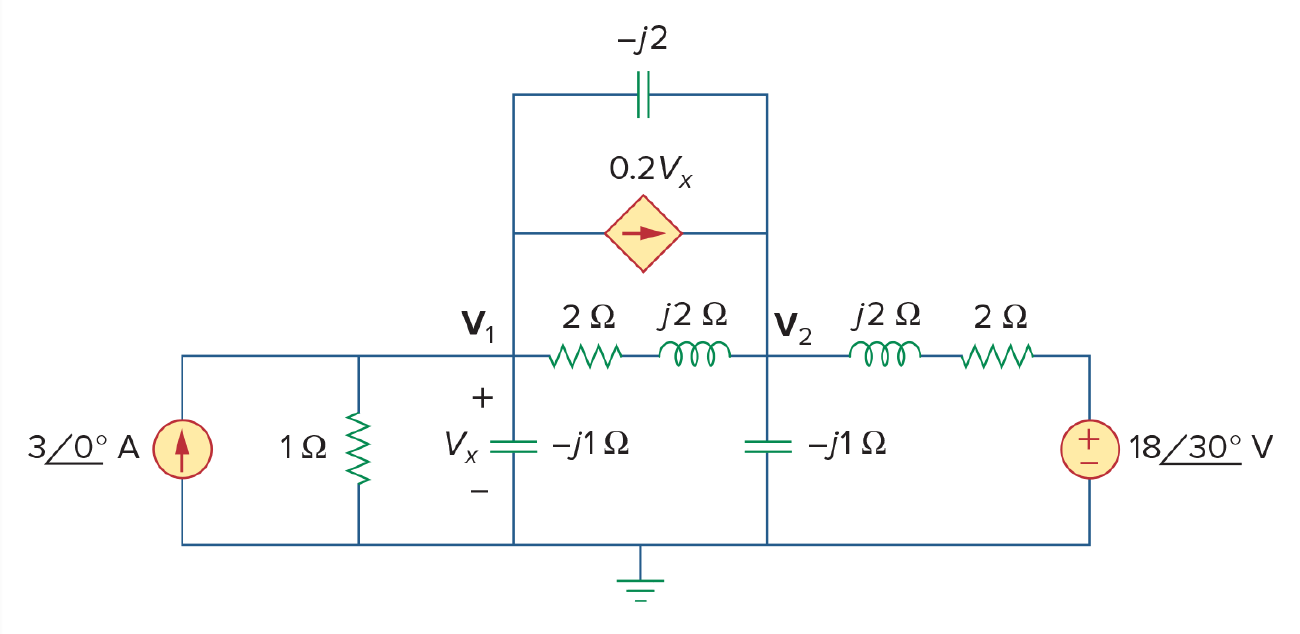
\includegraphics[width=127.1mm,max width=\linewidth]{../../assets/circuit/as7e1014.png}\end{center}
\begin{whybox}\textbf{\sffamily\color{navy}Why it is here.} Nine elements, three sources, one of them controlled by the voltage across a capacitor, and complex impedances on every branch. Nodal analysis by hand means complex algebra in two unknowns.\end{whybox}
\runhead{AC}
\begin{codebox}
\begin{Verbatim}[fontsize=\small]
j1,0,1,3
r1,1,0,1
rx,1,0,-1j
r3,1,2,-2j
j2,1,2,.2*vrx
r4,1,2,2+2j
r5,2,0,-1j
r6,2,3,2+2j
e,3,0,(18∠30°)
\end{Verbatim}
\end{codebox}
\settings{Analysis: AC, ω = 1 (any value gives the same answer, every impedance being in ohms). Rounding: 4 digits. Show AC answers as polar phasors.}
\begin{answerbox}
\adjustbox{max width=\linewidth}{$\displaystyle V_{1} = 2.708\angle{-56.73^\circ}\ \mathrm{V}$}
\end{answerbox}
\begin{answerbox}
\adjustbox{max width=\linewidth}{$\displaystyle V_{2} = 6.914\angle{-80.70^\circ}\ \mathrm{V}$}
\end{answerbox}
\applink{https://symbulator.pythonanywhere.com/?lesson=7&entry=10}
\end{problem}

\begin{problem}{Sample 6 of 12}{AS7's Example 12.11}{Three-phase wye-delta with line impedances}{Course, Lesson 9 (Three-Phase)}
{\itshape For the balanced Y-Δ circuit, find the line current $I_{aA}$, the phase voltage $V_{AB}$ and the phase current $I_{AC}$. The source frequency is 60 Hz.\par}
\vspace{1mm}
\begin{center}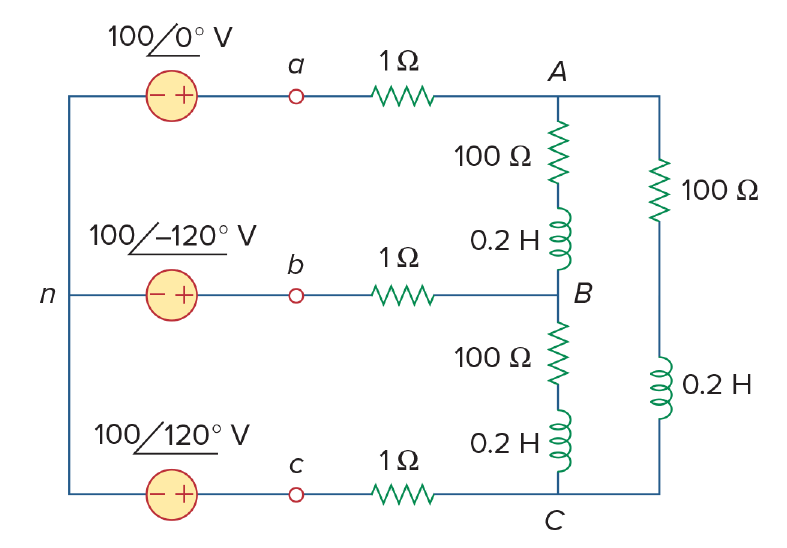
\includegraphics[width=89.0mm,max width=\linewidth]{../../assets/circuit/as7e1211.png}\end{center}
\begin{whybox}\textbf{\sffamily\color{navy}Why it is here.} The textbook converts the delta to a wye and works a single-phase equivalent. Symbulator needs neither: the three sources, the three lines and the delta go in as drawn.\end{whybox}
\runhead{AC}
\begin{codebox}
\begin{Verbatim}[fontsize=\small]
ea1,na1,0,100
eb1,nb1,0,(100∠-120°)
ec1,nc1,0,(100∠120°)
raa,na1,na2,1
rbb,nb1,nb2,1
rcc,nc1,nc2,1
rac,na2,nc2,100+24*pi*j
rcb,nc2,nb2,100+24*pi*j
rba,nb2,na2,100+24*pi*j
\end{Verbatim}
\end{codebox}
\settings{Analysis: AC, ω = 120π (60 Hz). Rounding: 4 digits. Polar phasors. Evaluate: vna2-vnb2.}
\begin{answerbox}
\adjustbox{max width=\linewidth}{$\displaystyle I_{aA} = i_{raa} = 2.350\angle{-36.20^\circ}\ \mathrm{A}$}
\end{answerbox}
\begin{answerbox}
\adjustbox{max width=\linewidth}{$\displaystyle V_{AB} = v_{na2}-v_{nb2} = 169.9\angle{30.81^\circ}\ \mathrm{V}$}
\end{answerbox}
\begin{answerbox}
\adjustbox{max width=\linewidth}{$\displaystyle I_{AC} = i_{rac} = 1.357\angle{-66.20^\circ}\ \mathrm{A}$}
\end{answerbox}
\applink{https://symbulator.pythonanywhere.com/?lesson=9&entry=6}
\end{problem}

\begin{problem}{Sample 7 of 12}{AS7's Practice Problem 13.13}{Coupled coils in a tangle}{Alexander \& Sadiku sampler}
{\itshape Find $i_o$ in the circuit of the figure.\par}
\vspace{1mm}
\begin{center}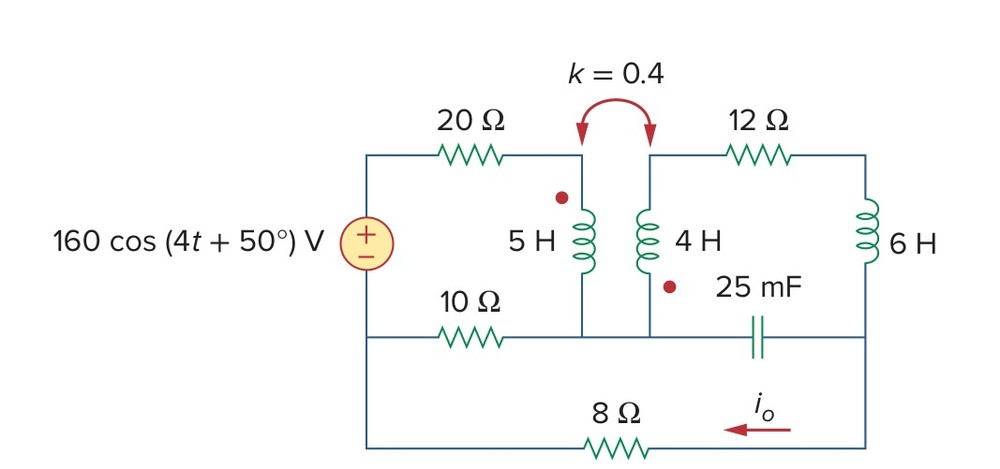
\includegraphics[width=132.2mm,max width=\linewidth]{../../assets/circuit/as7-pp13-13.jpg}\end{center}
\begin{whybox}\textbf{\sffamily\color{navy}Why it is here.} Two coils coupled by k = 0.4, dots at opposite ends, a third coil, and a capacitor hung from the node the coupled coils share. The coupling is one line naming the two coils.\end{whybox}
\runhead{AC}
\begin{codebox}
\begin{Verbatim}[fontsize=\small]
e,1,0,(160∠50°)
r20,1,a,20
l1,a,m,5
l2,m,b,4
m,l1,l2,k=0.4
r12,b,c,12
l3,c,r,6
c,m,r,25'm
r10,0,m,10
r8,r,0,8
\end{Verbatim}
\end{codebox}
\settings{Analysis: AC, ω = 4. Rounding: 4 digits. Polar phasors.}
\begin{answerbox}
\adjustbox{max width=\linewidth}{$\displaystyle i_{o} = i_{r8} = 2.011\angle{68.51^\circ}\ \mathrm{A}$}
\end{answerbox}
\applink{https://symbulator.pythonanywhere.com/?lesson=as7&entry=48}
\end{problem}

\begin{problem}{Sample 8 of 12}{NR11's switched RLC with coupled coils}{A transient across a coupling}{Course, Lesson 10 (Coupling)}
{\itshape A 48 V source feeds a 10 mF capacitor, a 4 Ω resistor and a 0.8 H coil in series. A switch across the capacitor has been closed a long time and opens at t = 0. The coil is coupled, M = 0.8 H, to a 1.6 H coil across a 20 Ω resistor. Find $v_o$, the voltage across the 20 Ω, for t > 0.\par}
\vspace{1mm}
\begin{center}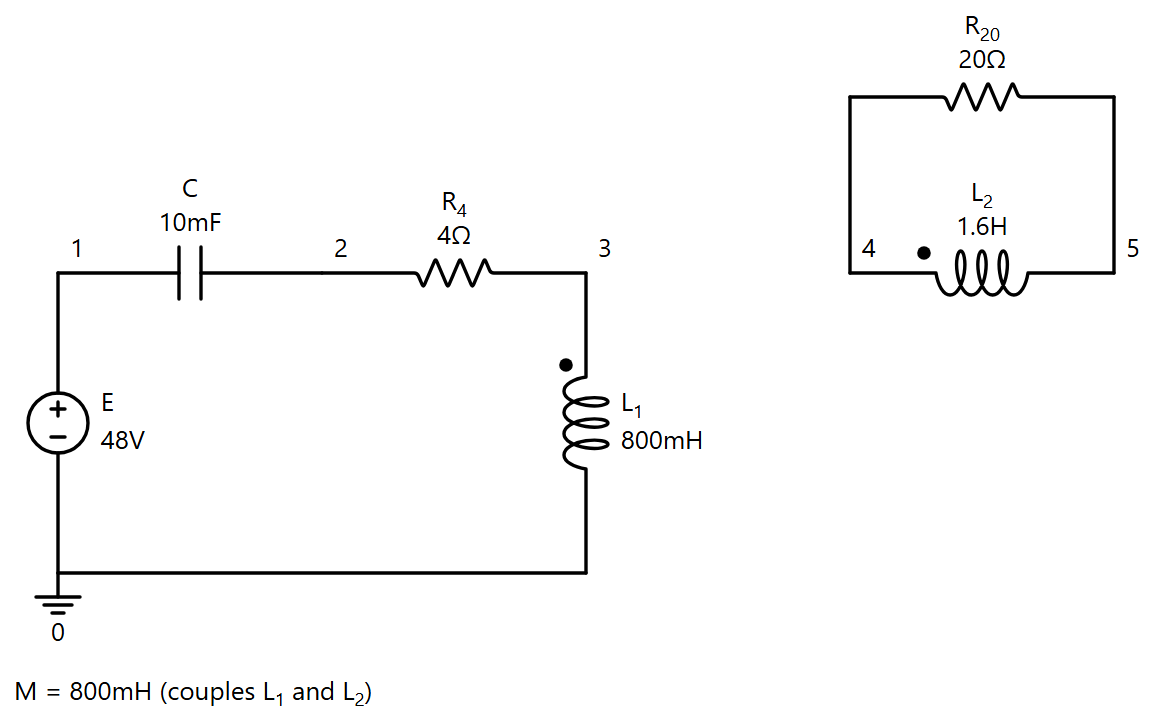
\includegraphics[width=99.2mm,max width=\linewidth]{../../assets/circuit/sym_nr11_coupled_capacitor.png}\end{center}
\begin{whybox}\textbf{\sffamily\color{navy}Why it is here.} A second-order primary talking to a first-order secondary through a mutual inductance. The answer carries both natural responses, an oscillation at 10 rad/s and a decay at 25 per second.\end{whybox}
\begin{minipage}[t]{0.485\linewidth}
\runhead{DC, t < 0}
\begin{codebox}
\begin{Verbatim}[fontsize=\small]
e,1,0,48
r4,1,3,4
l1,3,0,0.8
l2,4,5,1.6
r20,4,5,20
m,l1,l2,0.8
\end{Verbatim}
\end{codebox}
\settings{Analysis: DC.}
\begin{answerbox}
\adjustbox{max width=\linewidth}{$\displaystyle i_{l1} = 12\ \mathrm{A}$}
\end{answerbox}
\begin{answerbox}
\adjustbox{max width=\linewidth}{$\displaystyle i_{l2} = 0\ \mathrm{A}$}
\end{answerbox}
\applink{https://symbulator.pythonanywhere.com/?lesson=10&entry=17}
\end{minipage}\hfill
\begin{minipage}[t]{0.485\linewidth}
\runhead{TR, t > 0}
\begin{codebox}
\begin{Verbatim}[fontsize=\small]
e,1,0,48
c,1,2,10'm,0
r4,2,3,4
l1,3,0,0.8,12
l2,4,5,1.6,0
r20,4,5,20
m,l1,l2,0.8
\end{Verbatim}
\end{codebox}
\settings{Analysis: TR. Rounding: 4 digits. Evaluate: v4-v5.}
\begin{answerbox}
\adjustbox{max width=\linewidth}{$\displaystyle v_{o} = e^{-5t}\left(60\cos 10t - 120\sin 10t\right) - 60\,e^{-25t}\ \mathrm{V}$}
\end{answerbox}
\applink{https://symbulator.pythonanywhere.com/?lesson=10&entry=18}
\end{minipage}
\end{problem}

\begin{problem}{Sample 9 of 12}{Bo2's Drill Exercise 6.6}{Two capacitors around an op amp}{Course, Lesson 6 (Transients)}
{\itshape In the circuit, suppose that $v_S(t) = 2 - 2u(t)$ V. Find $v_o(t)$ for t ≥ 0.\par}
\vspace{1mm}
\begin{center}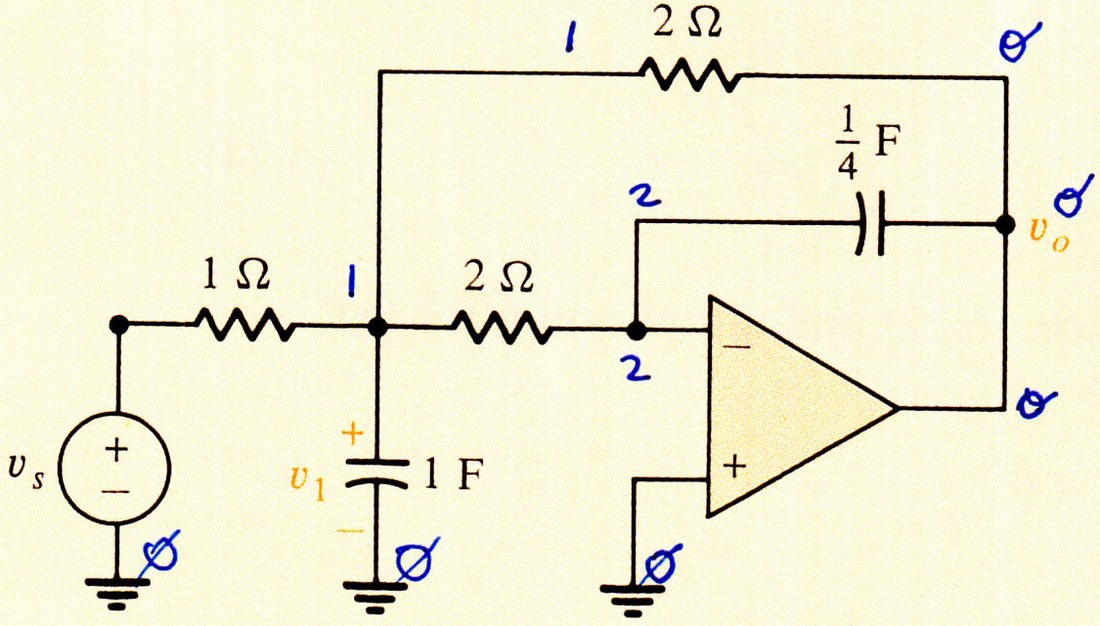
\includegraphics[width=108.9mm,max width=\linewidth]{../../assets/practice/bo2s-drill-exercise-6-6-op-amp-37.jpg}\end{center}
\begin{whybox}\textbf{\sffamily\color{navy}Why it is here.} An active second-order circuit whose two poles land in the same place. The repeated pole shows as the t in the answer, which no hand-picked solution form has to anticipate.\end{whybox}
\begin{minipage}[t]{0.485\linewidth}
\runhead{DC, t < 0}
\begin{codebox}
\begin{Verbatim}[fontsize=\small]
e,3,0,2
r1,3,1,1
r2,1,2,2
r3,1,o,2
ca,1,0,1
cb,2,o,1/4
o,0,2,o
\end{Verbatim}
\end{codebox}
\settings{Analysis: DC.}
\begin{answerbox}
\adjustbox{max width=\linewidth}{$\displaystyle v_{ca} = 0\ \mathrm{V}$}
\end{answerbox}
\begin{answerbox}
\adjustbox{max width=\linewidth}{$\displaystyle v_{cb} = 4\ \mathrm{V}$}
\end{answerbox}
\applink{https://symbulator.pythonanywhere.com/?lesson=6d&entry=7}
\end{minipage}\hfill
\begin{minipage}[t]{0.485\linewidth}
\runhead{TR, t > 0}
\begin{codebox}
\begin{Verbatim}[fontsize=\small]
r1,0,1,1
r2,1,2,2
r3,1,o,2
ca,1,0,1,0
cb,2,o,1/4,4
o,0,2,o
\end{Verbatim}
\end{codebox}
\settings{Analysis: TR.}
\begin{answerbox}
\adjustbox{max width=\linewidth}{$\displaystyle v_{o} = (-4t-4)\,e^{-t}\ \mathrm{V}$}
\end{answerbox}
\applink{https://symbulator.pythonanywhere.com/?lesson=6d&entry=8}
\end{minipage}
\end{problem}

\begin{problem}{Sample 10 of 12}{Prof. Boulet's exam problem}{The switch, the ladder and the damped sine}{Course, Lesson 6 (Transients)}
{\itshape The circuit comes from the circuits analysis class of Professor Eliane Boulet de Cabrera, at Universidad Tecnológica de Panamá. Find $v_1$ and $v$.\par}
\vspace{1mm}
\begin{center}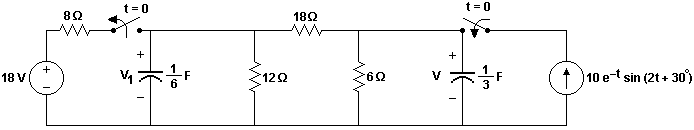
\includegraphics[width=183.6mm,max width=\linewidth]{../../assets/practice/a-more-complex-problem-44.png}\end{center}
\begin{whybox}\textbf{\sffamily\color{navy}Why it is here.} Two capacitors with their own initial conditions, and after the switch a current source that is itself a damped sinusoid. The answer holds two natural modes and a forced response. The TI calculator took 78 seconds and version 9 takes about one.\end{whybox}
\begin{minipage}[t]{0.485\linewidth}
\runhead{DC, t < 0}
\begin{codebox}
\begin{Verbatim}[fontsize=\small]
e,3,0,18
r8,3,1,8
ca,1,0,1/6
r12,1,0,12
r18,1,2,18
r6,2,0,6
cb,2,0,1/3
\end{Verbatim}
\end{codebox}
\settings{Analysis: DC. Rounding: exact.}
\begin{answerbox}
\adjustbox{max width=\linewidth}{$\displaystyle v_{ca} = 9\ \mathrm{V}$}
\end{answerbox}
\begin{answerbox}
\adjustbox{max width=\linewidth}{$\displaystyle v_{cb} = 9/4\ \mathrm{V}$}
\end{answerbox}
\applink{https://symbulator.pythonanywhere.com/?lesson=6d&entry=18}
\end{minipage}\hfill
\begin{minipage}[t]{0.485\linewidth}
\runhead{TR, t > 0}
\begin{codebox}
\begin{Verbatim}[fontsize=\small]
ca,1,0,1/6,9
r12,1,0,12
r18,1,2,18
r6,2,0,6
cb,2,0,1/3,9/4
j,0,2,10e^(-t)*sin(2t+30*pi/180)
\end{Verbatim}
\end{codebox}
\settings{Analysis: TR. Limit the results to v1, v2.}
\begin{answerbox}
\adjustbox{max width=\linewidth}{$\displaystyle \begin{aligned} v_{1} &= \left(\tfrac{5\sqrt{3}}{17}-\tfrac{20}{17}\right)e^{-t}\cos 2t - \left(\tfrac{20\sqrt{3}}{17}+\tfrac{5}{17}\right)e^{-t}\sin 2t \\ &\quad + \left(\tfrac{80\sqrt{3}}{17}+\tfrac{193}{34}\right)e^{-t/2} + \left(\tfrac{9}{2}-5\sqrt{3}\right)e^{-t}\ \mathrm{V}\end{aligned}$}
\end{answerbox}
\begin{answerbox}
\adjustbox{max width=\linewidth}{$\displaystyle \begin{aligned} v_{2} &= -\left(\tfrac{245\sqrt{3}}{34}+\tfrac{20}{17}\right)e^{-t}\cos 2t + \left(\tfrac{245}{34}-\tfrac{20\sqrt{3}}{17}\right)e^{-t}\sin 2t \\ &\quad + \left(\tfrac{80\sqrt{3}}{17}+\tfrac{193}{34}\right)e^{-t/2} + \left(\tfrac{5\sqrt{3}}{2}-\tfrac{9}{4}\right)e^{-t}\ \mathrm{V}\end{aligned}$}
\end{answerbox}
\applink{https://symbulator.pythonanywhere.com/?lesson=6d&entry=19}
\end{minipage}
\end{problem}

\begin{problem}{Sample 11 of 12}{AS7's Problem 19.2}{A two-port with no ground}{Course, Lesson 13 (Two-Ports)}
{\itshape Determine the impedance parameters of the ladder: four 1 Ω resistors in the upper rail, four in the lower, three 1 Ω rungs.\par}
\vspace{1mm}
\begin{center}
\begin{circuitikz}[scale=0.85, transform shape, american]
\draw (0,3) node[ocirc, label=left:\textcolor{accent}{a}]{}
  to[R=1\,$\Omega$, -*] (2.5,3) node[above right, text=accent]{b}
  to[R=1\,$\Omega$, -*] (5,3)   node[above right, text=accent]{c}
  to[R=1\,$\Omega$, -*] (7.5,3) node[above right, text=accent]{d}
  to[R=1\,$\Omega$, -o] (10,3)  node[right, text=accent]{e};
\draw (0,0) node[ocirc, label=left:\textcolor{accent}{f}]{}
  to[R, l_=1\,$\Omega$, -*] (2.5,0) node[below right, text=accent]{g}
  to[R, l_=1\,$\Omega$, -*] (5,0)   node[below right, text=accent]{h}
  to[R, l_=1\,$\Omega$, -*] (7.5,0) node[below right, text=accent]{i}
  to[R, l_=1\,$\Omega$, -o] (10,0)  node[right, text=accent]{j};
\draw (2.5,3) to[R=1\,$\Omega$] (2.5,0);
\draw (5,3)   to[R=1\,$\Omega$] (5,0);
\draw (7.5,3) to[R=1\,$\Omega$] (7.5,0);
\end{circuitikz}
\end{center}
\begin{whybox}\textbf{\sffamily\color{navy}Why it is here.} Eleven resistors and no node 0 anywhere. Each port is written as its pair of terminals, so the lower rail stays in the circuit instead of being shorted to ground.\end{whybox}
\runhead{DC}
\begin{codebox}
\begin{Verbatim}[fontsize=\small]
r1,a,b,1
r2,b,c,1
r3,c,d,1
r4,d,e,1
r5,f,g,1
r6,g,h,1
r7,h,i,1
r8,i,j,1
r9,b,g,1
r10,c,h,1
r11,d,i,1
\end{Verbatim}
\end{codebox}
\settings{Analysis: Find equivalent, Two-port parameters, z, between [a,f] and [e,j]. Rounding: 4 digits.}
\begin{answerbox}
\adjustbox{max width=\linewidth}{$\displaystyle z_{11} = z_{22} = 41/15 = 2.733\ \Omega$}
\end{answerbox}
\begin{answerbox}
\adjustbox{max width=\linewidth}{$\displaystyle z_{12} = z_{21} = 1/15 = 0.06667\ \Omega$}
\end{answerbox}
\applink{https://symbulator.pythonanywhere.com/?lesson=13&entry=14}
\end{problem}

\begin{problem}{Sample 12 of 12}{NR12's Example 18.6}{Two amplifiers known only by their h parameters}{Nilsson \& Riedel sampler}
{\itshape Two identical amplifiers are connected in cascade. Each is described by its h parameters: $h_{11}$ = 1000 Ω, $h_{12}$ = 0.0015, $h_{21}$ = 100, $h_{22}$ = 100 µS. The source has 500 Ω of internal resistance and the load is 10 kΩ. Find the voltage gain $V_2/V_g$.\par}
\vspace{1mm}
\begin{center}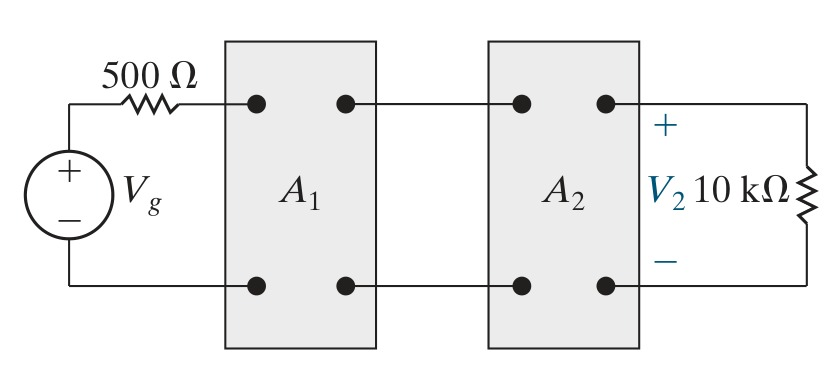
\includegraphics[width=139.3mm,max width=\linewidth]{../../assets/circuit/nr12-ex18-6.jpg}\end{center}
\begin{whybox}\textbf{\sffamily\color{navy}Why it is here.} Each amplifier is a single element carrying its four parameters, and the cascade is two lines sharing a node. No matrix products, no conversions between parameter sets.\end{whybox}
\runhead{DC}
\begin{codebox}
\begin{Verbatim}[fontsize=\small]
e,1,0,vg
rs,1,a,500
h1,a,b,[1000,0.0015,100,0.0001]
h2,b,c,[1000,0.0015,100,0.0001]
rl,c,0,10'k
\end{Verbatim}
\end{codebox}
\settings{Analysis: DC. Rounding: approx. Evaluate: v\_c/vg.}
\begin{answerbox}
\adjustbox{max width=\linewidth}{$\displaystyle V_{2}/V_{g} = v_{c}/v_{g} = 33333.33$}
\end{answerbox}
\applink{https://symbulator.pythonanywhere.com/?lesson=nr12&entry=16}
\end{problem}

\begin{problem}{Bonus}{A freebie, on the house}{One dependent source of each kind}{Course, Lesson 3 (Sources), as the Showing-off Problem}
{\itshape Find positive values for $V_s$ and $I_s$ that will result in 80 W delivered by the VCCS and 0 W dissipated in the CCVS.\par}
\vspace{1mm}
\begin{center}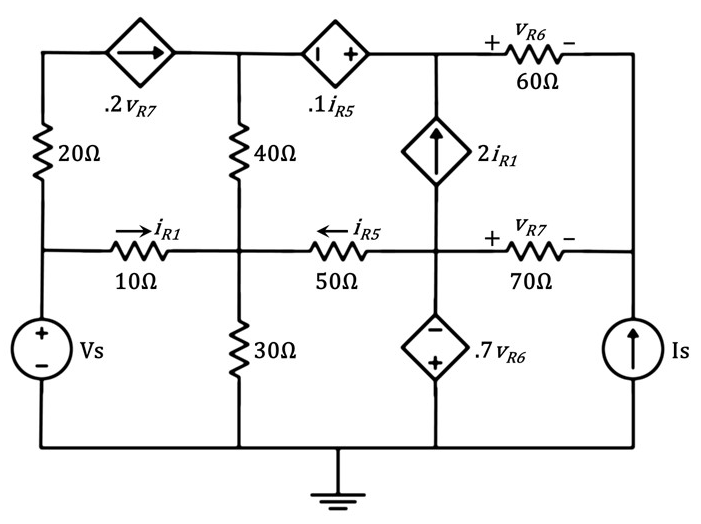
\includegraphics[width=82.9mm,max width=\linewidth]{../../assets/practice/the-showing-off-problem-expert-4.png}\end{center}
\begin{whybox}\textbf{\sffamily\color{navy}Why it is here.} Invented by Roberto Perez-Franco in 2013 to show off. A VCCS, a CCVS, a CCCS and a VCVS woven through seven resistors, and the question runs backwards, from powers to sources. The two power conditions are quadratic, so four solutions fit, and the conditions pick the positive one. The answers also show why the CCVS dissipates nothing: its controlling current is exactly zero.\end{whybox}
\runhead{DC, Expert Mode}
\begin{codebox}
\begin{Verbatim}[fontsize=\small]
es,e,0,vs
js,0,d,is
r1,e,m,10
r2,a,e,20
r3,m,0,30
r4,b,m,40
r5,n,m,50
r6,c,d,60
r7,n,d,70
jd1,a,b,0.2vr7
ed2,c,b,0.1ir5
jd3,n,c,2ir1
ed4,0,n,0.7vr6
\end{Verbatim}
\end{codebox}
\settings{Analysis: DC. Rounding: 4 digits. Expert Mode: equations pjd1 = -80 and ped2 = 0, unknowns vs, is, conditions vs > 0 and is > 0.}
\begin{answerbox}
\adjustbox{max width=\linewidth}{$\displaystyle v_{s} = 17.61\ \mathrm{V}$}
\end{answerbox}
\begin{answerbox}
\adjustbox{max width=\linewidth}{$\displaystyle i_{s} = 0.3973\ \mathrm{A}$}
\end{answerbox}
\begin{answerbox}
\adjustbox{max width=\linewidth}{$\displaystyle i_{r5} = 0\ \mathrm{A}$}
\end{answerbox}
\applink{https://symbulator.pythonanywhere.com/?lesson=3&entry=49}
\end{problem}

\end{document}
